\section{Watchdog Feature}
\label{sec:watchdog}

The watchdog feature is a component that stops testing after a defined time. It is necessary because the AskoziaPBX does not respond
any more if it reaches its limit. Is is implemented like that:

\begin{figure} [!ht]
\centering
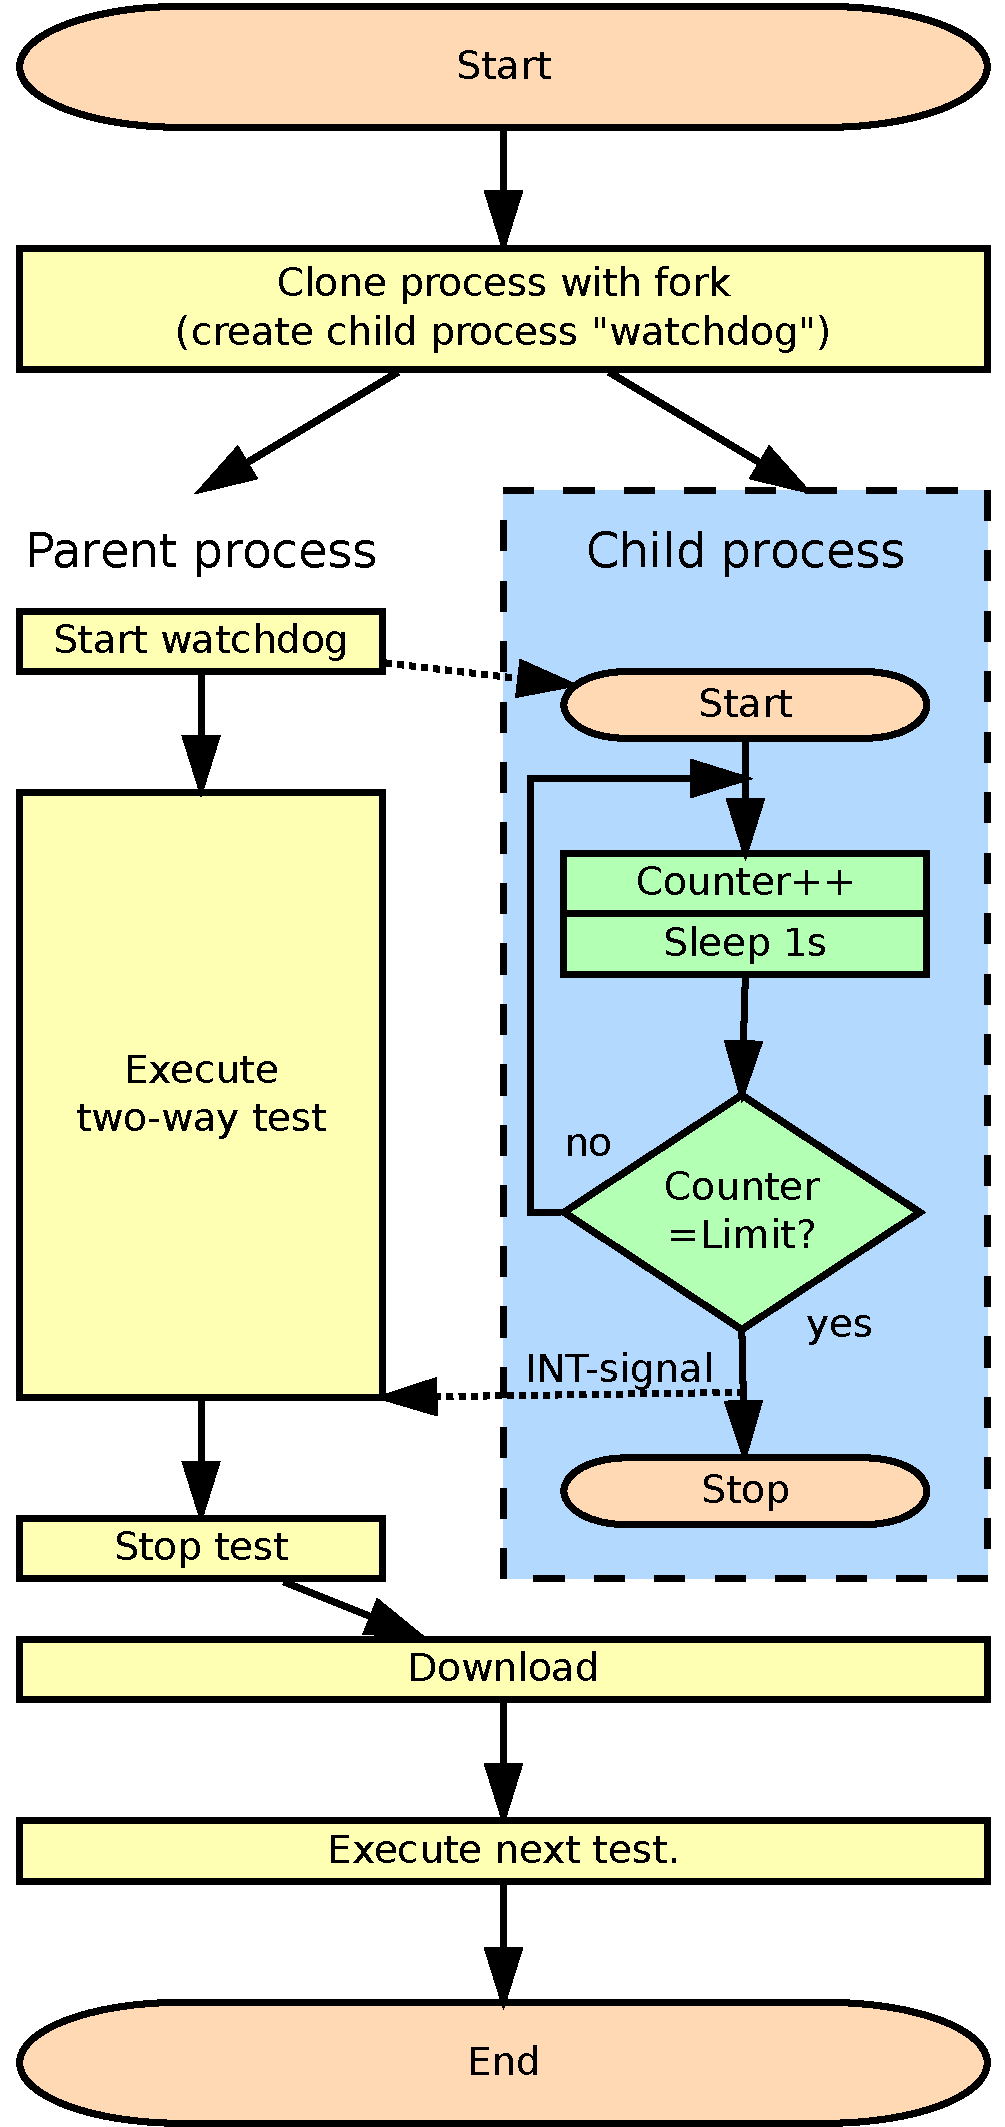
\includegraphics [width=8cm] {watchdog-1}
\caption{Basic watchdog process}
\label{fig:watchdog-basic-process}
\end{figure}

\newpage
Of course, it is not as easy as it is shown in figure~\ref{fig:watchdog-basic-process}. First of all,
there is only one watchdog process that is forked before beginning the tests.
This process is started and stopped multiple times (one time for every test type):

\begin{figure} [!ht]
\centering
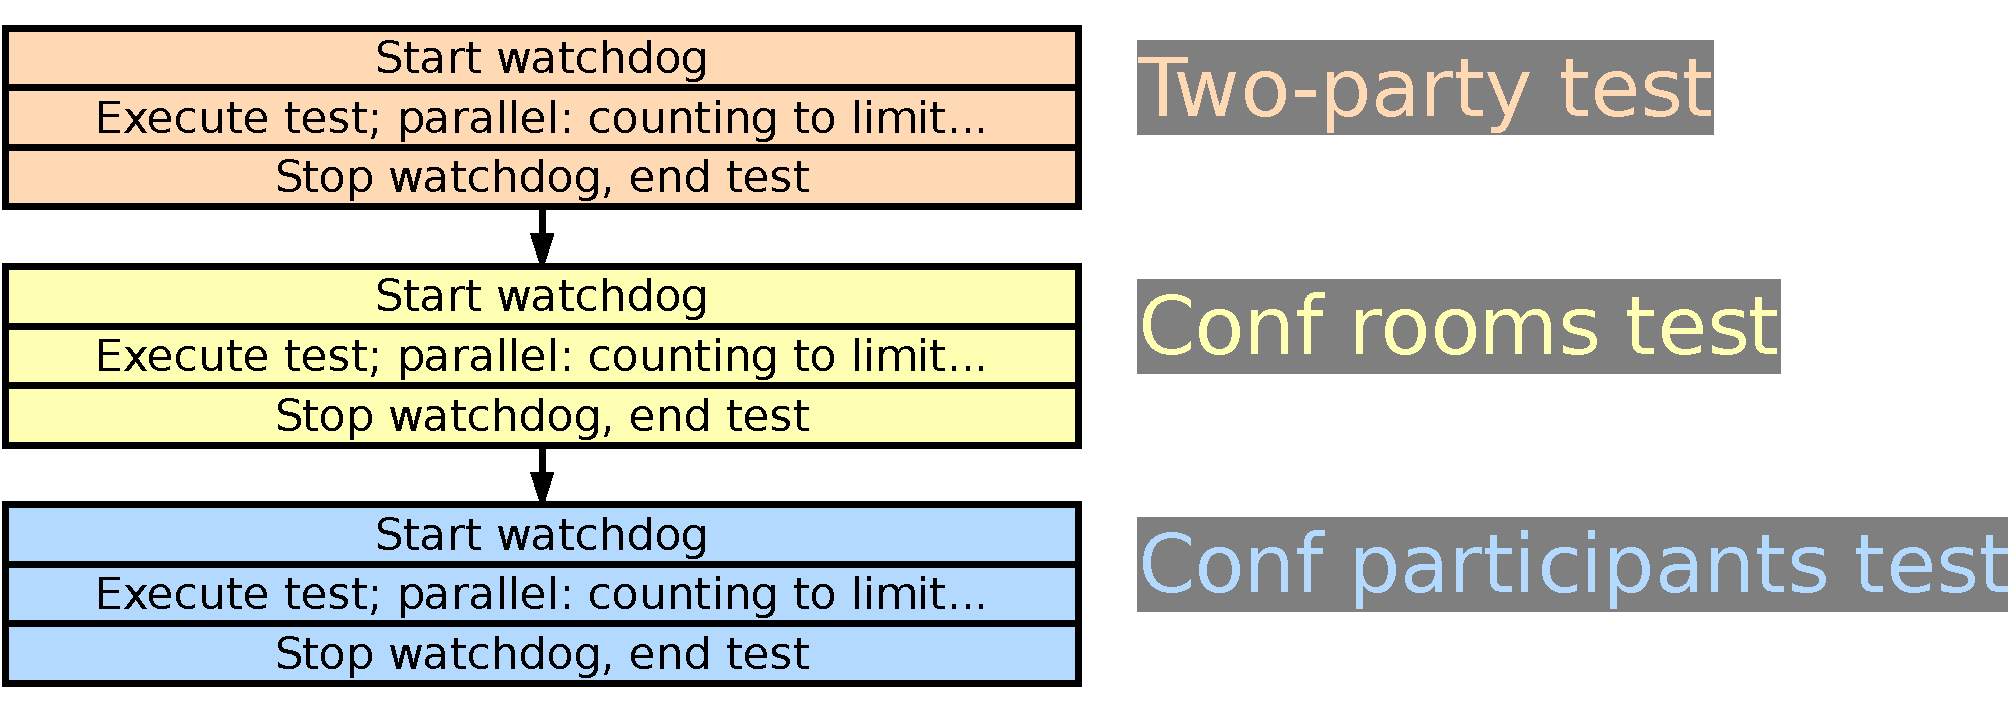
\includegraphics [width=14cm] {watchdog-2}
\caption{Starts and stops of watchdog}
\end{figure}

Let's sum up: Now there is a second process that is started before every test and stopped after every test.
At the end of all tests, it is killed. But there is still one problem: Because of the variable parameters,
the tests may have very different durations. So, it is necessary to tell the watchdog some settings of the test.
For this reason, there is an IPC (Interprocess Communication) existing. After forking the main process, there
is a pipe created to send messages from the parent (test) process to the child (watchdog). It can be treated
like a normal print device in perl, so it is possible to send messages like this:

\begin{lstlisting}[breaklines=true,label=code:watchdog-pipe,caption={Send messages to watchdog} ]
print $pipe $message;
\end{lstlisting}

It is possible to send to following commands to the watchdog. All commands have to end with a newline character
for flushing the pipe:

\begin{tabular}{|p{3.5cm}|p{10.5cm}|} \hline
\textsc{Testtype} & \textsc{Needed users} \\ \hline \hline
\texttt{set pause '3'}		& Set pause time to 3 seconds \newline (necessary for call duration calculation) \\
\texttt{set users '5'}		& Set number of users to 5 \newline (necessary for call duration calculation) \\
\texttt{start watchdog}		& Starts watchdog: Begin of incrementing counter per second \\
\texttt{stop watchdog}		& Stops watchdog (incrementing counter) \\
\texttt{Tests finished.}	& Terminates watchdog process. \\
\hline
\end{tabular}

After sending a command, the counter is reset to zero automatically (there is no provision for sending commands
to the watchdog while running a test). Sometimes, there were problems if two commands are sent in quick succession, 
so it is recommended to sleep one second between sending two commands.

